
%%%%%%%%%%%%%%%%%%%%%%%%%%%%%%%%%%%%%%%%%%%%%%%%%%%%%%%%%%%%%%%%%%%%%%%
%\chapter{On Gnuscope}
%\label{GnuscopeUse}
%%%%%%%%%%%%%%%%%%%%%%%%%%%%%%%%%%%%%%%%%%%%%%%%%%%%%%%%%%%%%%%%%%%%%%%

\chapter{Overview}

Gnuscope was created as the latest of the group of programs based on Scope Fit (SF) which have been used, maintained, and improved by Dr. Tabor and his students.  It deviates from prior versions of SF in several important ways.  First, Gnuscope is written using the GNU (GNU is not Unix) Image Manipulation Program (GIMP) Tool Kit (GTK) and Drawing Kit (GDK), and therefore the Gnuscope interface is independent of other programs~\ref{gnuscopeinterface}.  Prior versions of SF relied on the Tektronics 4010 terminal emulation to display spectra~\ref{sfgraphics}.  Second, Gnuscope was written in the C programming language while prior versions of SF used the FORTRAN programming language.  Additionally, the user interface for Gnuscope is driven by pull-down menus and accelerator keys while prior versions of SF relied on accelerator keys only.  The use of pull-down menus makes Gnuscope easier to use for beginners.  Finally, Gnuscope handles memory in a fundamentally different way than prior versions of SF.  Prior versions of SF allocated memory at compile time.  As a direct consequence, a new version of SF was required for each large data structure.  In contrast, Gnuscope allocates memory for each large data structure as needed.  Therefore, a single program can handle multiple large data structures without overwhelming the computer.  In short, Gnuscope deviates from prior versions of SF by using GTK and GDK, being written in C, using pull-down menus, and using dynamic memory allocation.

\begin{figure}[h]
\begin{center}
\scalebox{0.5}{
\includegraphics{gnuscopeinterface.ps}
}
\caption{\label{gnuscopeinterface}The Gnuscope interface displaying 3 spectra.}
\end{center}
\end{figure}

\begin{figure}
\begin{center}
\scalebox{0.5}{
\includegraphics{sfgraphics.ps}
}
\caption{\label{sfgraphics}Scope Fit's graphical display.}
\end{center}
\end{figure}

Despite the differences with prior versions of SF, Gnuscope maintains backwards compatibility with prior versions of scope fit.  For instance, Gnuscope can read all file formats from prior versions of Scope Fit (and then some).  Additionally, the accelerator keys for functions in Gnuscope are the same as the accelerator keys in prior versions of SF wherever possible.  

\chapter{Basic Use}
\section{Command Line Options}

Even before Gnuscope has started, the user has the option to provide it input.  This is done by the command line functions.  A summary of command line functions can be displayed using the {\it -h} flag from the command line.  At the time of this writing the following options were available.

\subsection{Read File}

syntax:
\begin{verbatim}
gnuscope --file $<$filename$>$
gnuscope -f $<$filename$>$
\end{verbatim}
This option allows the user to start Gnuscope with data in memory.  All file types supported by the automatic file recognition system are allowed.  This option can be particularly powerful when combined with a command file.
\subsection{Help}

\begin{verbatim}
gnuscope -h
\end{verbatim}
This provides a list of the currently available command line functions.

\section{Program Defaults and Configuration Files}

In recognition that many of its defaults are not always the best choice for analyzing all data, Gnuscope can use configuration files.  It begins by looking for a file with the name {\bf .gnuscopeconfig} in the local directory, and if and only if it does not find it it will look for the same file in the user's home directory.  If Gnuscope does not find a configuration file, or the configuration file which it finds does not override its defaults, it will use its defaults (Gah! that was an awkward sentence).  The current options for a configuration file are as follows.

\subsection{Comments - $\#$}

To make sure that you can remember why you are by default reading a file, or starting with a particular display configuration you can insert comments into a configuration file by starting a line with the $\#$ symbol.

\subsection{Read File - {\it in}}

There are cases where you might want to start with a particular set of files in memory.  For example if you use a particular directory to analyze a certain matrix you might want to always start by reading that matrix and its total projection.  You may use the same wild-card characters as you do from the command prompt.

\subsection{Set Histogram Mode - {\it Display Mode}}

The four options for {\it Display Mode} are {\it Linear}, {\it Log}, {\it Root}, and {\it EffCor}.  These control the way the histograms are displayed.  The only one which is not fairly self explanatory is {\it EffCor}.  {\it EffCor} will try to correct for detector efficiency once the energy and efficiency calibrations have been entered (which cannot be easily done in the configuration file.  Otherwise it behaves just like {\it Linear}.

\subsection{Set Y-Scale Overlay Mode - {\it OverlayYScaleMode}}

Gnuscope can use two methods to determine the relative vertical scales when overlaying histograms.  {\it OverlayYScaleMode 0} will cause Gnuscope to use the same vertical scale for all overlayed histograms.  The vertical scale is set so that the first histogram, which is colored black, has its highest peak at 90$\%$ of the histogram.  If {\it OverlayYScaleMode} is set to 1, Gnuscope will determine the vertical scale for each of the overlayed histograms independently so that each histogram is displayed at 90$\%$ of the vertical space.

\subsection{Set Polynomial Degree for 2D Display Interpolation - {\it Set2DPoly}}

{\it Set2DPoly} is used to determine the polynomial degree for the interpolation in the two dimensional plot.  If {\it Set2DPoly} is set to 0 it will turn off the interpolation.  Unfortunately, there are some issues with interpolation.  The major problem is that it takes time.  The amount of time it takes to render a histogram increases rapidly with the degree of interpolation.  The other problem is that odd polynomial degrees can cause bazaar effects at the edge of the display.  Because of these two problems, the Polynomial degree should be set to 0 or 2 for most purposes.

\subsection{Set 2D Display Color Mode - {\it DensityPlotColors}}

The density plots can be rendered in {\it Color} or {\it BW}.  {\it Color} is recommended for on screen viewing.  However, if only a black and white printer is available for hardcopies, {\it BW} is superior.

\subsection{Set 2D Display Type - {\it DensityPlotType}}

Gnuscope can display density plots as {\it Density} plots, {\it Contour} plots, or {\it DensityAndContour} plots.  

\subsection{Set 2D Contour Mode - {\it ContourMode}}

There are five ways Gnuscope determines the placement of the contours when displaying 2D histograms, {\it Linear}, {\it Log}, {\it Root}, {\it InverseLog}, and {\it InverseRoot}.  {\it Linear} sets the isobar values so they are equally spaced from the minimum value to the maximum value.  {\it Log} sets the isobar values so the Log of the isobars' value are equally spaced between the Log of the minimum value and the maximum value.  {\it Root} sets the isobar values so the square roots of the isobars are equally spaced.  {\it InverseLog} and {\it InverseRoot} are the same as {\it Log} and {\it Root} except that the isobar values range from the max to the min instead of the other way around.

\subsection{Set Number of 2D Contours - {\it NumContours}}

{\it NumContours} will set the number of contour lines displayed on the in the {\it Contour} and {\it DensityAndContour} modes.

\section{Interface}

Once Gnuscope has started, the screen should be pretty much covered by a single window.  This window should look like other windows on the Gnome Desktop (or KDE).  The pull-down menus are at the very top, and the channel information is directly below it.  Just below that is a text widget for output.  There are probably some messages to users in this window about possible changes.  To the right of the text is a graphic.  If the user doesn't like the graphic they may simply click on it and it will vanish.  Finally, below the text window is the display area.

While this window is active, the user may access functions by using either the pull down menus or by using the accelerator keys.  In addition to the accelerator keys listed in the pull-down menus, the user may jump to one of the first nine spectra by pressing the corresponding key on the keyboard.  They may also goto the next or previous spectrum by pressing the up or down arrow key, shift the display to the right or left by using the corresponding arrow key, scale the range up or down using the {\it Page Up} and {\it Page Down} keys, and adjust the binning by using the {\it Home} and {\it end} keys.  Also, markers are set by clicking.

Gnuscope can display up to sixteen spectra at the same time.  This can be accomplished by simply selecting more than one spectra in the {\it Display} function.  When displaying more than one spectrum, Gnuscope assumes that the last spectrum clicked is the one which the analysis and display functions should be applied to.

\chapter{File Types}

In order to have greatest compatibility with other programs, Gnuscope can read and write many file types.  In order to determine the file type Gnuscope looks at the file extension.  Unfortunately, if the file extension is incorrect problems can occur; therefore, if the user is experiencing difficulty reading a particular file, they should check the file extension.  At the time of this writing it could read many one dimensional file types, two file types for density plots, four file types for matrices, a slew of setup files for various sorting options, Gnuscope specific command files, and a configuration file.  The are summarized below.

\section{Spectra Files}

Spectrum files are used to store individual spectra.  They come in many varieties, and Gnuscope can read and write binary and ASCII SF spectrum files, DAMM spectrum files, GF3 (radware) spectrum files, and generic ASCII spectrum files.  Additionally, Gnuscope can extract the spectrum data from GENIE data files and SpecTCL data files and write lipha data files.  As mentioned previously, Gnuscope uses the file extension to determine the file type when reading and writing files and the file extension corresponding to each file type is given after it's name below.  When writing files, Gnuscope defaults to binary {\it Nuclear Spectrum Files} and will write the data in this format if no valid file extension is given.

 \subsection{Nuclear Spectrum Files (.NSM)}

Nuclear Spectrum Files (NSM) are the default histogram file type for both prior versions of Scope Fit and Gnuscope.  Each file contains a small amount of metadata about the file and about each spectrum.  The format of the file is a file header ({\it fh}) followed by a data header ({\it dh}) and data ({\it D}) for each spectrum.  So for $n$ spectra in a NSM file the format would look like.

\begin{equation}
fh,dh_1,D_1,dh_2,D_2,...,dh_n,D_n
\end{equation}

The file header is 33 bytes long and its structure is shown in Fig.~\ref{nsmfileheader}.  Because the original versions of Scope Fit were written in Fortran, it begins and ends with an four byte integer, labeled {\it Buffer} in the figure, which says that it has twenty-five bytes of actual information.  The first two bytes of which are the run number.  After that, another two bytes contain the number of spectra in the file.  Then, four bytes contain the truetime for the run.  Next, nine bytes contain the date of the run.  Finally, eight bytes contain the time of the run.

\begin{figure}
\addcontentsline{toc}{figure}{Nuclear Spectrum file header}
\begin{center}
\scalebox{.5}{
\rotatebox{-90}{
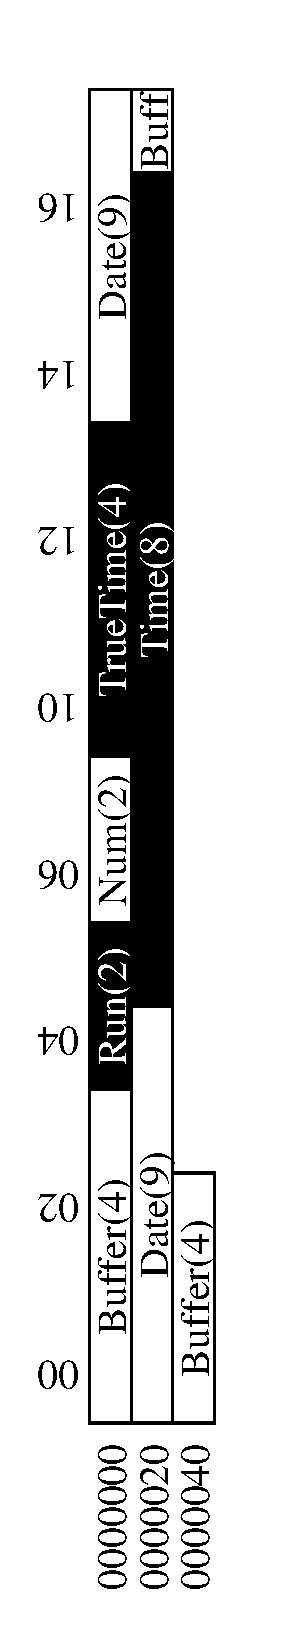
\includegraphics{nsmfileheader.ps}}}
\caption{\label{nsmfileheader}The structure of the file header for nuclear spectrum files.  The memory address to the left of the diagram is in octal, as would be shown in Octal Dump (od).  To aid the reader, the memory regions alternate between black on white and white on black and each label has the number of bytes that region occupies.}
\end{center}
\end{figure}

A data header is twenty-two bytes long and its structure is shown in Fig.~\ref{nsmdataheader}.  As with the file header it begins and ends with a four byte integer showing how much information is actually in the buffer, in this case 12 bytes.  The first piece of actual data is a two byte integer showing the number of channels for that spectrum.  The number of channels is the number of data points in the subsequent data part of the file.  Next, two bytes show the itype, which is retained for backwards compatibility, but for Gnuscope should always be 2.  Then, six bytes are reserved for a six character title for the plot.  Finally, the truetime for that spectrum is stored in the last four bytes of actual data.

\begin{figure}
\addcontentsline{toc}{figure}{Nuclear Spectrum file data header}
\begin{center}
\scalebox{.5}{
\rotatebox{-90}{
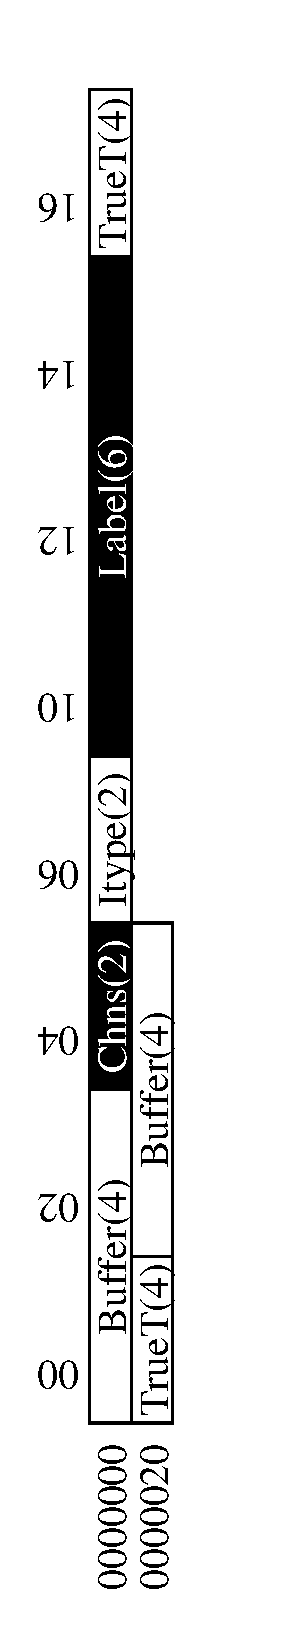
\includegraphics{nsmdataheader.ps}}}
\caption{\label{nsmdataheader}The structure of the data header for nuclear spectrum files.  The memory address to the left of the diagram is in octal, as would be shown in Octal Dump (od).  To aid the reader, the memory regions alternate between black on white and white on black and each label has the number of bytes that region occupies.}
\end{center}
\end{figure}

Finally, the actual data is stored as integers in a single buffer.  As with the other buffers, it begins and ends with an integer containing its length.

 \subsection{ASCII Nuclear Spectrum Files (.nsm)}

ASCII nuclear spectrum files are related to, but not exactly binary NSM files.  They lack metadata such as truetime, time, and date.  They can also be substantially less compact than their binary cousins.  An ASCII nuclear spectrum writes out an id number, the size, the title, and the data for each run.  There is no universal header or obvious divisions between the spectra.  An ASCII NSM file with a small and uninteresting spectra might look like this.

{\small
\begin{verbatim}
1 15 SPECTRA
1 2 3 4 5 6 7 8 9 10 11 12 13 14 15

\end{verbatim}
}

 \subsection{DAMM Spectrum Files (.spk)}

The default file type for histograms from the DAMM.  As with the binary NSM file the file begins with a file header, {\it fh}, which contains a small amount of metadata about the rest of the file followed by data headers, {\it dh}, and data, {\it D}.  Unlike NSM files, if there are more than 254 spectra in a file, there is a need for a second file header.  If there are more than 512 spectra there is a need for a third file header and so on..  A SPK file would have the general structure of

\begin{equation}
fh,dh_1,D_1,dh_2,D_2,...,dh_{254},D_{254},fh,dh_{255},D_{255},...,dh_n,D_n.
\end{equation}


The file header for a DAMM spectrum file contains somewhat less information that that for the NSM file.  The structure of the DAMM file header is shown in Fig.~\ref{spkfileheader}.  It begins with eight bytes which contain the data type.  Then, there is a four byte integer containing the number of spectra in the file.  Next, there is another four bytes which shows the location of the next file header in half-words.  In this case half-words are 2 byte units.  Finally, there is a listing of the spectra id's and locations in half-words.

\begin{figure}
\addcontentsline{toc}{figure}{DAMM spectrum file header}
\begin{center}
\scalebox{.5}{
\rotatebox{-90}{
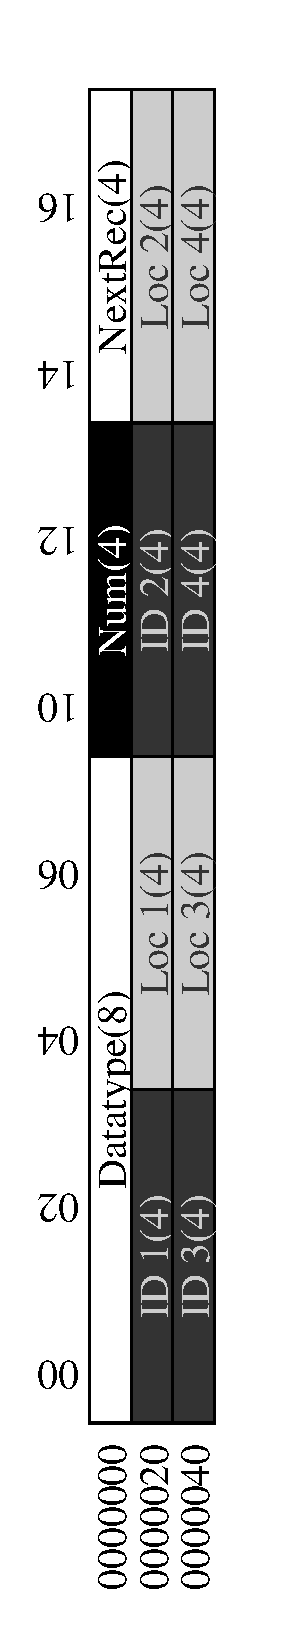
\includegraphics{spkfileheader.ps}}}
\caption{\label{spkfileheader}The structure of the data header for DAMM spectrum file.  The memory address to the left of the diagram is in octal, as would be shown in Octal Dump (od).  To aid the reader, the memory regions alternate between black on white and white on black and each label has the number of bytes that region occupies.}
\end{center}
\end{figure}

The data header structure for the DAMM spectrum files is shown in Fig.~\ref{spkdataheader} and begins with a four-byte integer containing the {\it ID} of the spectrum.  After that, there are twelve bytes containing a character {\it Label} for the spectrum and a second twelve byte character string containing the {\it Timestamp} for the spectrum.  Then, there is an obsolete four-byte integer labeled {\it Bytes} which should always be set to -4.  Next, there is another four-byte integer containing the {\it Length} of the data header in two byte words.  As luck would have it this is always sixty-four.  Subsequently, there are two obsolete four-byte integers which are labeled {\it Datalength} and {\it Dimensions} in Fig.~\ref{spkdataheader}.  {\it Datalength} can be any value, but {\it Dimensions} should be 1.  Next, there are three four-byte integers with similar information, {\it Channels}, {\it Raw}, and {\it Scaled}.  {\it Channels} is the number of channels in the histogram.  {\it Raw} is the number of raw channels in the histogram, and {\it scaled} is the number of channels in the spectrum after the calibration is applied.  After the information about the numbers of channels there are two four-byte integers, {\it MinChan} and {\it MaxChan}, which are the first and last non-zero channel in the spectrum.  Then, there are three four byte floats for the {\it Constant}, {\it Linear}, and {\it Quadratic} calibration constants.  Finally, there are eight bytes of {\it Reserved Space} followed by forty bytes for a character string containing the {\it Title} of the spectrum.  The data for the spectrum follows its header as four-byte integers.

\begin{figure}
\addcontentsline{toc}{figure}{DAMM spectrum file data header}
\begin{center}
\scalebox{.5}{
\rotatebox{-90}{
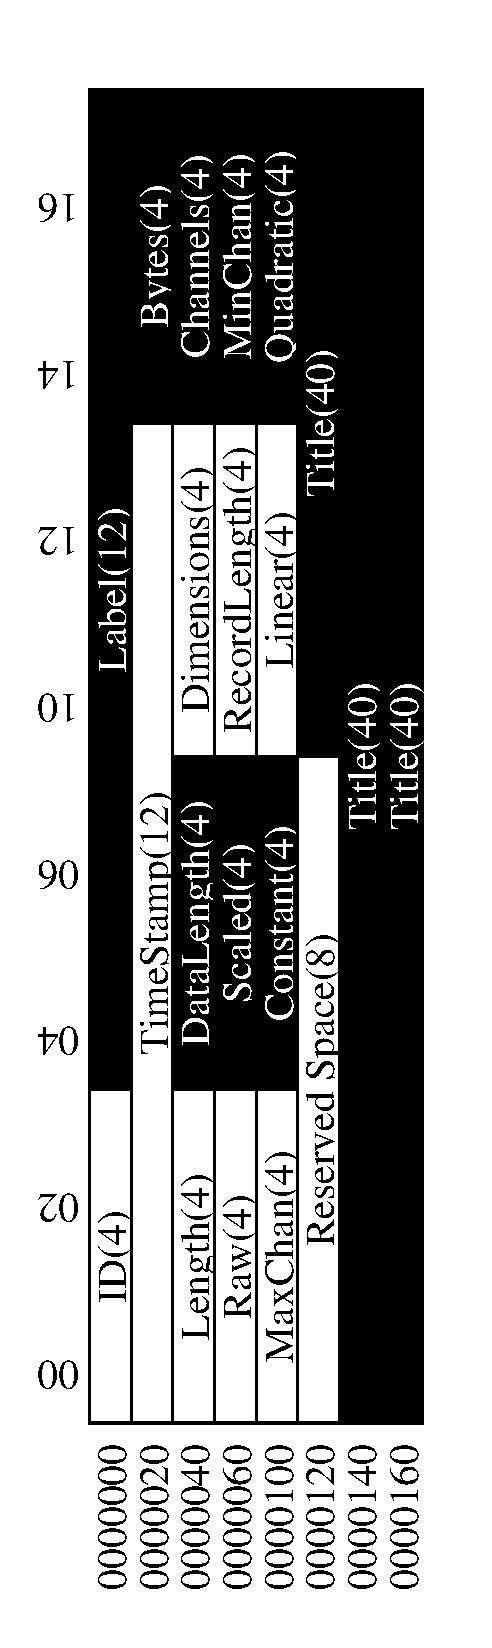
\includegraphics{spkdataheader.ps}}}
\caption{\label{spkdataheader}The structure of the data header for DAMM spectrum file.  The memory address to the left of the diagram is in octal, as would be shown in Octal Dump (od).  To aid the reader, the memory regions alternate between black on white and white on black and each label has the number of bytes that region occupies.}
\end{center}
\end{figure}

 \subsection{Radware Spectrum Files (.spe)}

The default file type for histograms from Radware.

SPE files are ASCII, not binary and do not have a file header.  The data headers begin with a nine character field for the title, followed by the size of the spectrum and three ones, each occupying ten bytes.  Finally, the data for the spectrum is listed eight channels at a time each occupying ten bytes.  A short SPE file might look something like this.

{\tiny
\begin{verbatim}
Run 0 TT:        24         1         1         1
         1         2         3         4         5         6         7         8
         9        10        11        12        13        14        15        16
        17        18        19        20        21        22        23        24
\end{verbatim}
}

 \subsection{GENIE spectrum files (.cnf or .CNF) - {\it READ ONLY}}

Gnuscope can extract the histograms from GENIE data files but cannot read any of the metadata from the GENIE data files.  Each GENIE data file contains a single histogram.  This means that reading in a large number of GENIE data files can be quite tedious.  However, the command line flag {\it -f} can use wildcards and can be used to read in many GENIE data files at once (Ex. gnuscope -f *.cnf).  At the present time, Gnuscope cannot write GENIE data files.  Because of the Digital Copyright Millennium Act the method for extracting the spectrum from a CNF file will not be discussed in this document.

 \subsection{Generic ASCII Files (.txt)}

A new file type for inputting and exporting histograms in a simple way.  The format is a two column text file.  The first column is the x value and the second column is the y value.  When reading, Gnuscope assumes a new histogram has started when the x value decreases.  For instance, a generic ASCII file containing two very short and meaningless spectra would look like this.

\begin{verbatim}
1 1
2 2
3 3
4 4
5 5
6 6
7 7
8 8
9 9
10 10
1 10
2 9
3 8
4 7
5 6
6 5
7 4
8 3
9 2
10 1
\end{verbatim}

\section{SpecTCL spectrum files (.asc) - {\it READ ONLY}}

SpecTCL, the data acquisition software at the National Superconducting Cyclotron Laboratory (NSCL) at Michigan State University (MSU) can output a spectrum file in an ASCII format.  Gnuscope can read in these files, but currently cannot read them in.  Because of this limitation the format of these files will not be discussed here, but an interested party can look to the SpecTCL webpage, http://sourceforge.net/projects/nsclspectcl/.

 \subsection{LIPHA data files (.dat) - {\it WRITE ONLY}}

Gnuscope can be used to generate a general ASCII file with the appropriate metadata for them to be used as LIPHA data files from the displayed region of the most recently clicked graph.  To do this access the {\bf Write Lipha} option from the {\bf File} pull-down menu.  Gnuscope cannot read these files.  For more information about LIPHA and the files it uses please refer to \underline{http://www-highspin.phys.utk.edu/~hjin/download.html}.

\section{Density Plot Files}

These files are used to store data from density plots.  The ASCII density plot file can accommodate one density plot, while the binary version can accommodate as many as needed.

 \subsection{ASCII Density Plot File (.big)}

The ASCII version of the density plot file is very wasteful of disk space, however, it is easily readable by a human.  The format consists of two numbers separated by a comma.  These are the x and y dimension of the density plot.  These are followed by rows of ten numbers, separated by commas, which contain the channel information progressing first in the x direction, then in the y direction.  For example, the ASCII density plot file which would result in Fig.~\ref{bigfileexample} would look like this.

\begin{verbatim}
10,10
1,2,3,4,5,6,7,8,9,10
11,12,13,14,15,16,17,18,19,20
21,22,23,24,25,26,27,28,29,30
31,32,33,34,35,36,37,38,39,40
41,42,43,44,45,46,47,48,49,50
51,52,53,54,55,56,57,58,59,60
61,62,63,64,65,66,67,68,69,70
71,72,73,74,75,76,77,78,79,80
81,82,83,84,85,86,87,88,89,90
91,92,93,94,95,96,97,98,99,100
\end{verbatim}

\begin{figure}
\addcontentsline{toc}{figure}{A sample ASCII density plot file}
\begin{center}
\scalebox{.5}{
\rotatebox{90}{
\includegraphics{bigfileexample.ps}}}
\caption{\label{bigfileexample}A simple density plot file generated by hand using the ASCII density plot file format.}
\end{center}
\end{figure}

 \subsection{Binary Density Plot file (.ede)}

The binary version of the density plot file is somewhat more compact than its ASCII counterpart, but is still uncompressed.  Its main advantages are its ability to store more than one plot at a time and the space for a text label.  The file format consists of an integer showing the number of density plots contained as a four-byte integer.  Next, each density plot is is written as 80 bytes of characters, one integer for the x dimension, one integer for the y dimension, and then the channel information as integers as is shown in Fig.~\ref{ededataheader}.


\begin{figure}
\addcontentsline{toc}{figure}{The binary density plot header}
\begin{center}
\scalebox{.5}{
\rotatebox{-90}{
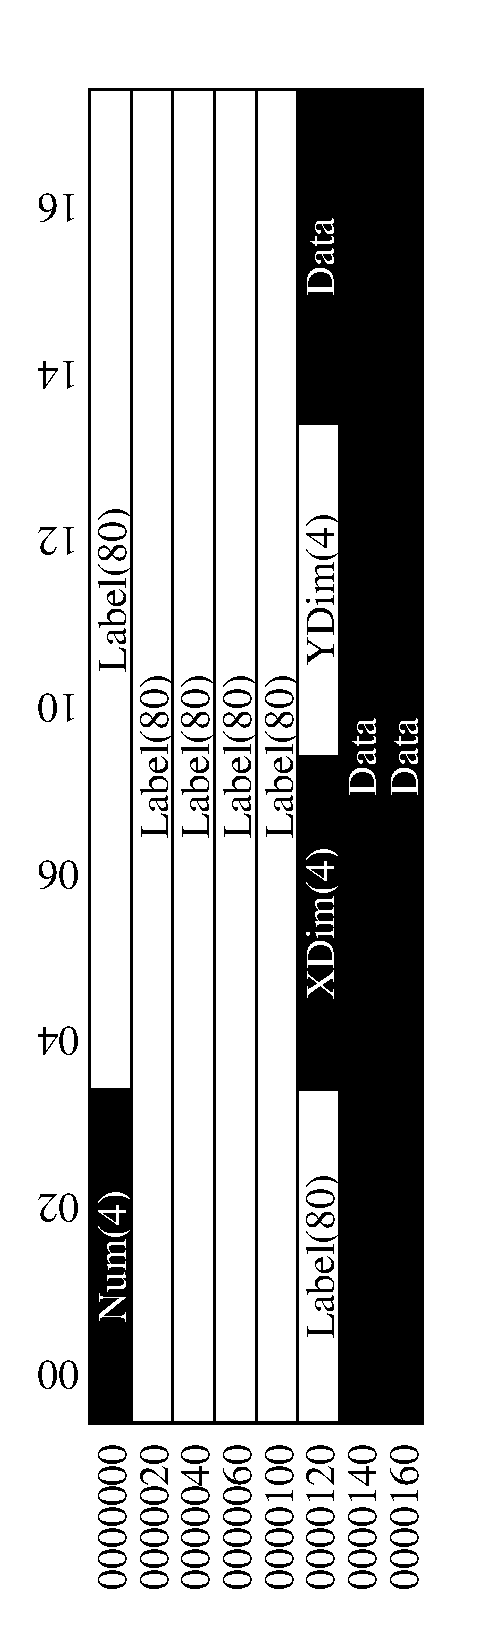
\includegraphics{ededataheader.ps}}}
\caption{\label{ededataheader}A schematic of what the the octal dump of a binary density plot file would look like.  With the exception of the leading four bytes, labeled {\it num}, this information is repeated for each density plot in the file.}
\end{center}
\end{figure}

\section{Matrix Files}

The files for matrices come in a couple of varieties.  They can vary by the way the channel information is stored (float or short int), or they can vary by assumptions about symmetry.  Gnuscope tries to handle the identification of the float or short int variations automatically by looking at the beginning of the file.  Additionally, Gnuscope recognizes both matrices with no assumptions (.sqr) and those with symmetry assumed (.twd).  In the former case, each the number of counts for each combination of x and y coordinates is stored separately.  In the later, a little more than half the information is stored, with the assumption that the number of counts for (x$_0$,y$_0$) is the same as that for (y$_0$,x$_0$).  In order to save memory resources, the data for symmetric matrices is stored as a single array with the index determined by
\begin{equation}
Index = x - y + (size - y) * (y / 2).
\end{equation}
where {\it x} is the x coordinate, {\it y} is the y coordinate, and {\it size} is the number of channels on each side of the matrix.

\section{Sorting and Setup Files}

Gnuscope can also be used to sort data.  Currently, it can sort data from two different sources.  First, it can sort data gathered using the FSU Pittsburgh Gamma Array in either the .evt or the .ev2 compressed data formats.  Second, Gnuscope can be used to sort the presorted data from the GS92 run at {\sc Gammasphere}.  Unfortunately, the methods for sorting the two types of data differ greatly in ease of use.  Because Gnuscope was not used extensively to analyze GS92 data, the interface for sorting GS92 data is quite primitive and relies on a terminal.  Conversely, the interface for sorting data gathered at FSU is graphical, but requires more complex setup files.  Both methods of sorting use different files for the information they are supposed to sort.  These are summarized as follows:

First, let us examine the files used when sorting the GS92 data.

\subsection{GS92 Files}
\begin{itemize}
\item{Detector Information Files}

When the user wants to make a file with different detectors represented on each axis, they will have to use a Detector Information File.  This file should have the following format:
\begin{verbatim}
2
10
5 7 8 9 10 11 12 13 14 16
110 
1 2 3 4 5 6 7 8 9 10 11 12 13 14 15 16 17 18 19 20
21 22 23 24 25 26 27 28 29 30 31 32 33 34 35 36 37 38 39 40
41 42 43 44 45 46 47 48 49 50 51 52 53 54 55 56 57 58 59 60
61 62 63 64 65 66 67 68 69 70 71 72 73 74 75 76 77 78 79 80
81 82 83 84 85 86 87 88 89 90 91 92 93 94 95 96 97 98 99 100
101 102 103 104 105 106 107 108 109 110
\end{verbatim}
The first line is the compression, or the linear calibration for the final spectrum.  The second line is the number of detectors on the x axis, the third line is a space separated list of the ADC numbers for those detectors.  After that, the number of detectors on the y axis followed by a space separated list of the detectors on the y axis.

\item{Gamma Gate Files}

A gamma gate file is used to setup add and subtract gates during sorting.  The format is as follows.

\begin{verbatim}
1  738 745     494
1  1183 1187   790
1  587 596     395
1  471 476     315
1  484 488     325
1  1109 1119   743
1  1230 1237   823
1  1269 1274   847
1  1484 1493   993
1  637 645     428
0 0 0
\end{verbatim}

Each line represents a different gate.  The first item is the add or subtract gate flag (1 = add, -1 = subtract).  The second and third numbers are the upper and lower channel numbers for that gate.  The fourth number is a comment for the gamma ray which is represented by that gate.  The file should end in a line with three zeros.


Now let us examine the files which may be used when sorting data gathered at the FSU Pittsburgh Gamma Detector Array.

\end{itemize}

\subsection{PGAM Sort Files}

Pgamsort always requires at least two setup files, a master setup file (.msf) and a normal setup file (.sf) both of which are automatically recognized by Gnuscope.  The reason for the master setup file is to allow the data files (.evt or .ev2) to reside anywhere on the system and to allow different runs to have different setup files.  The normal setup file contains information about each ADC, which detectors are elements of multi-segment detectors, which detectors are part of particle telescopes, and which ADC channels correspond to TACs as well as what they monitor.  The format of these files will be covered shortly.  The different sorting options for pgamsort may require additional files, and these files will be discussed after the setup files.

\begin{itemize}

\item{Master Setup Files (.msf)}

As mentioned before the purpose of the master setup file is to twofold.  First, it allows the user to access data stored anywhere on the system.  Second it allows the user to have different setup files for different runs.  Let us look at an example.

\begin{verbatim}
/usr/users/pavan/experiment/c13be10/data/
2
101,101
/usr/users/pavan/experiment/c13be10/analysis/c13be10.sf
103,110
/usr/users/pavan/experiment/c13be10/analysis/c13be10-2.sf
ev2
\end{verbatim}

The first line is the path of the data files.  The data files should be in that location with filenames of the form run\#\#.evt or run\#\#.ev2 where \#\# is the run number.  The second line is the number of setup files which will be used.  After this the information about each setup file is entered.  The first of these lines is a comma separated list of the first run number and the last run number for that setup file.  The second line is the name of the setup file, including the path if you do not run Gnuscope from that directory.  The same setup file can be used more than once.  Finally, the {\it ev2} string at the end of the file tells Gnuscope to sort {\it ev2} files instead of evt files.  If the {\it ev2} string is not at the end of the file, Gnuscope assumes that the data is in the evt format.

\item{Setup Files (.sf)}

Setup files are used to provide information about the individual ADC channels and the types of detectors attached to each one.  Let us look at an example.

\begin{verbatim}
3000
2,0
8
E-1
1,8192,0
0,0.3859,0
E-DE-TAC
2,8192,0
0,1,0
CL1Red
5,8192,90
-0.1055,0.4985521,-4.642786e-07
CL1Green
6,8192,90
-1.043721e-01,4.985492e-01,-4.625999e-07
CL1Blue
7,8192,90
1.080196,4.983898e-01,-4.907510e-07
CL1Black
8,8192,90
-4.445766e-01,4.994469e-01,-4.496888e-07
TAC-DE-G
19,8192,0
0,1,0
DE-1
21,8192,0
0,1,0
2
DE1-E1
1,21,0.5,28
EvsTAC
1,2,0,29*
1
CL1
4,25
5,6,7,8
1
DE-G-TAC
19
4
5,1535,2488
6,1556,2579
7,1570,2824
8,1549,3623
\end{verbatim}

The first line is the number of channels for the final histograms and matrices.  The second line is the compression in keV per channel and the beta of the recoiling nuclei.  The third number is the number of ADCs which are to be used during sorting.  Note that this is the number of ADCs monitored during sorting, not the number of ADCs used in the experiment.  After that the information for each of those ADCs must be provided. 

 For each ADC three lines are required.  The first line is simply the text label for that ADC.  The second line is the ADC number, the maximum number of channels for that ADC, and the angle relative to the beam for the detector attached to the ADC separated by commas.  The last line is the constant, linear, and quadratic coefficients for the quadratic polynomial describing the relationship between channel and energy for that detector separated by commas.

  After the information for each of the ADCs has been entered the number of E-$\Delta$E telescopes must be entered.  If there are none put zero, but if you have particle telescopes you must now enter the appropriate information.  Each entry consists of two lines.  The first line is the text label of the particle telescope.  The second line is the ADC number of the E detector, the ADC number of the $\Delta$E detector, the relative gain, and a unique virtual ADC number separated by commas.  The virtual ADC number can be any positive integer, but it is advised that it isn't too big.  If the virtual ADC number is the same as another ADC which is in use, both spectra will appear in that histogram.  There are several options when entering information for a particle telescope.  First, if the user includes the * character in the line (beginning or ending) Gnuscope will not exclude the ADCs entered for the E and $\Delta$E from gamma and energy spectra.  This could be useful when looking at E$_\gamma$ vs TAC.  Second the user can include supplemental ADCs for the purposes of addback for either the E or the $\Delta$E ADC.  To do this the user simply puts them in parenthesis immediately after the first ADC (ex. 3(1,17) if 3 is the main ADC, and 1 and 17 are supplemental). 

 Next, the number of multi-segment germanium detectors is entered.  If there are no multi-segment germanium detectors in use, enter zero.  If there are multi-segment germanium detectors, there must be information about them three lines at a time.  The first line of this entry is the text description of the multi-segment detector.  The second line is the number of ADCs used by that detector and a virtual ADC number for the add-back result separated by commas.  The third line should be a comma separated list of the ADC numbers for this detector.  

Then, we can enter the number of TACs that are in use.  If there are no TACs in use enter zero.  If there are TACs in use enter a text label on the first line, the ADC number of the TAC on the second line, the number of other ADCs monitored by the TAC on the third line, and then list the range of the acceptable TAC signal for each of those ADCs.  The range of the acceptable TAC signal is entered as a comma separated list of the ADC number of the monitored signal and the lower and upper limits in channels for the TAC.  

Finally, there is the ability to enter options.  Currently there is only the option to set the size of the two dimensional histograms by adding a line containing EDESIZE followed by the desired resolution.

Because there is a large amount of information in a setup file, the user can test a particular setup file by attempting to read it after starting Gnuscope in an Xterm (or another console).  If the setup file is faulty, the output in the xterm should allow the user to determine the problem.

\item{Gamma Gate File}

Like with GS92 sorting, additional gamma gates can be placed during a sort.  Such a file is read during the sorting process and the file name is entered from the sorting window.  Gnuscope makes no assumptions about the file name containing gamma gates and does not automatically detect them.  In the case of PGAM sort, the file format for gamma gating is slightly different from sorting GS92 data.  For example:

\begin{verbatim}
3
779 782
905 915
1245 1254
\end{verbatim}

The first line is the number of gamma gates.  The next lines are space separated upper and lower limits for additive gates in units of energy.

\item{Veto Gate File}

In some cases you want to reject events with a particular signal.  This can be done in Gnuscope using a the Veto Gate option.  To use this option a file must be entered in the PGAM sort window.  Gnuscope makes no assumptions about the file name and cannot automatically detect these files.  A veto gate file would look like:

\begin{verbatim}
1,4092,8192
3,4092,8192
2,4092,8192
17,4092,8192
20,4092,8192
\end{verbatim}

Each line consists of a comma separated list of the ADC number and the lower and upper channels to veto.

\item{Required Signal File}

In some cases you might only want events with a particular signal.  In this case you can use the Requires Signal option in the PGAM sort window.  This will require a file identical in format to the {\it Veto Gate} option.

\item{Axis Information File}

As with sorting GS92 data, PGAM sort can be used to create a matrix with one set of detectors represented on one axis and another set of detectors represented on the other.  To do this the user must input a Axis Information file of the same format as with the GS92 sort (please refer there) in the PGAM sort window.  Gnuscope makes no assumptions about the names of these files and cannot automatically detect them.

\item{Pair Information File}

Used to generate matrices in which data is only written on an axis if a particular pair of detectors fires.  Used when measuring polarization.  A file consists of the ADC numbers of each signal in the format (a,b).

\item{Particle Gate File}

The file format for {\it Particle Gates} is very similar to that of the {\bf BIG} file.  The integer for each file corresponds to a bit map with a 1 in a bit for each particle telescope included in that gate.

\item{Calibration Info File}

A Calibration Info File should contain a two column list of the energies and intensities from a radioactive source.  They columns should be separated by spaces.

\end{itemize}

\section{Command Files}

Command files are a very powerful tool.  At the time of this writing they have not been used extensively in Gnuscope.  However, Gnuscope supports them and the available commands are summarized below.

\begin{itemize}

\item{Read File - in $<$filename$>$}

When the command file interpreter reads this line it will read the file designated by $<$filename$>$ using the standard Gnuscope read function.  Wildcards can be used in the filename to read in more than one file at once.

\item{Set Calibrations - cal $<$histogram \#$>$ $<$a$>$ $<$b$>$ $<$c$>$}

When the command file interpreter reads this line it will set the energy calibrations for the spectrum designated by the $<$histogram \#$>$.  The first time this is done the global assumptions about energy calibrations are set.  After that, they are only set for the designated spectrum.

\item{Set Markers - mark $<$channel$>$}

When the command file interpreter reads this line it will place a mark at the designated channel number.

\item{Set Background - background $<$counts$>$}

When the command file interpreter reads this line it will set the background to the counts designated in the command.

\item{Sum - sum $<$minchan$>$ $<$maxchan$>$ $<$background$>$}

When the command file interpreter reads this it will return information about the number of counts between $<$minchan$>$ and $<$maxchan$>$ inclusive.

\item{Gaussian Fit - gauss $<$minchan$>$ $<$maxchan$>$ $<$background$>$}

When the command file interpreter reads this line it will make a Gaussian fit to the data between $<$minchan$>$ and $<$maxchan$>$ assuming $<$background$>$.

\item{Fixed FWHM Gaussian Fit - fixedFWHMgauss $<$minchan$>$ $<$maxchan$>$ $<$background$>$ $<$FWHM$>$}

When the command file interpreter reads this line it makes a Gaussian fit to the data between $<$minchan$>$ and $<$maxchan$>$ assuming both a fixed $<$FWHM$>$ and $<$background$>$.

\item{Double Gaussian Fit - doublegauss $<$minchan$>$ $<$maxchan$>$ $<$center1$>$ $<$center2$>$ $<$FWHM1$>$ $<$FWHM2$>$ $<$background$>$}

The command file interpreter will attempt to perform a double Gaussian fit on the data between channels $<$minchan$>$ and $<$maxchan$>$ it assumes that $<$center1$>$ and $<$center2$>$ are approximately the centers of the peaks, that they are approximately $<$FWHM1$>$ and $<$FWHM2$>$ wide, respectively, and that $<$background$>$ is the background.

\item{Exponential Fit - expfit $<$minchan$>$ $<$maxchan$>$}

The command file interpreter will tell gnuscope to make an exponential fit to the data between $<$minchan$>$ and $<$maxchan$>$.

\item{Sorting}

Sorting via a command file involves a lot of commands.  The procedure for sorting this way should be to issue a clear command, set your options, then issue a sort command.  An example will follow the list of commands.

\begin{itemize}

\item{Clear Sorting Parameters - sort sort}

Clears out the sorting parameters.

\item{Turn TAC Output On - sort output tac}

Toggles the TAC output on.  This will also toggle the {\it Energy Histogram} output off.

\item{Turn Energy Histogram Output On - sort output histogram}

Toggles the energy histogram output on.  This will also toggle the {\it TAC output} off.

\item{Turn On Density Plot Output - sort output part $<$opt telescope zoom$>$}

This will turn on the two dimensional histogram output.

\item{Turn On $\gamma$-$\gamma$ Symmetric Matrix Output - sort output twd}

This will toggle on a symmetric matrix for $\gamma$-$\gamma$ events.  It will also toggle off all other matrix outputs.

\item{Turn On $\gamma$-$\gamma$ Matrix Output - sort output ggsqr $<$filename$>$}

This will toggle on a matrix for $\gamma$-$\gamma$ events.  The filename should be a {\bf Detector Gate File} describing which detectors should be on each axis.Toggling this on will also toggle off other matrix outputs.

\item{Turn On Particle-$\gamma$ Matrix Output - sort output pgsqr $<$final particle energy calibration$>$}

The command file interpreter will toggle on the particle-$\gamma$ matrix output.  The user should include the final energy calibration for the particle axis.  Toggling this output method on will turn off the other matrix output modes.

\item{Turn On $\gamma$ Pair Matrix Output - sort output pairsqr $<$filename$>$}

When the command file interpreter reads this it will toggle on a matrix consisting of pairs. The user should provide a filename for the {\bf Pair Information File}.  Toggling this on will toggle off the other matrix outputs.

\item{Turn On TAC gating - sort gate tac}

TAC gating can be toggled on by issuing the {\it sort gate tac} command in the command file.

\item{Turn On Particle Gating - sort gate part $<$opt filename$>$}

The command line interpreter will toggle particle gating on when it reads this line.  The user may provide a file name for a {\bf Particle Gate File}.

\item{Turn On Gamma Gating - sort gate gamma $<$minchan$>$ $<$maxchan$>$}

This will turn on gamma gating.  The user needs to provide both a minimum channel and a maximum channel for the gamma gate.

\item{Turn On Gamma Gating using a file - sort gate gamma $<$filename$>$}

The will turn on gamma gating.  The user needs to provide a file name for a {\bf Gamma Gate File}.

\item{Turn On Veto Selection - sort gate veto $<$filename$>$}

This line will cause the command file interpreter will turn on veto gating.  The user needs to provide a file name for a {\bf Veto Gate File}.

\item{Turn On Required Signal Selection - sort gate requires $<$filename$>$}

The command line will interpret this as turning on the required signal gating.  The user must provide a file name for the {\bf Required Signal File}.

\item{Turn On Clover Self Suppression - sort gate selfsuppressclovers}

The command file interpreter will turn on clover self suppression if this line is included.

\item{Turn On Clover Minimum Multiplicity - sort gate minmultipolarity $<$min$>$}

The command file interpreter will interpret this by toggling on the clover minimum multipoloarity with $<$min$>$ as the minimum multipoloarity.

\item{Start Sorting - sort sort}

This causes the command file interpreter to start sorting.

\end{itemize}
\end{itemize}

\chapter{Menu Functions}

\section{File}

This is the menu for file operations.  They are listed below.

\subsection{Read}

Read is used to input files.  It uses a primitive automatic file detection method, looking at the file extension.  Currently, the file types summarized in the File Types section are recognized unless otherwise noted.  If there are spectra in memory the user will be asked if they want to retain the spectra currently in memory.  Once answering this question they will be able to use a standard Gnome file selection dialog to select the file to read.

\subsection{Write Histograms}

If the user wants to save the spectra currently in memory they can use this function.  They will be asked for the first and last spectra to write to file.  Then they will be able to select the file to write to using a standard Gnome file selection dialog.  The file type is automatically detected by the extension.  If no extension is given Gnuscope assumes the NSM file type and adds that file extension to the file name.

\subsection{Write Lipha}

When making a spectrum figure for a paper, this is a very useful function.  When called the user will select the file to which to write, and then Gnuscope will write a LIPHA data file from the currently displayed data in the active spectrum.

\subsection{Write 2D Histograms}

If there are two dimensional histograms in memory, usually E vs. $\Delta$E plots, this function can be used to save them.  As with the {\it Write Histograms} function it looks to the file extension to determine the file type.  In this case the choices are {\bf .big} and {\bf .ede}.  The latter is the assumed file type and if the file extension is not given it will be used and the {\bf .ede} file extension is concatenated to the file name.

\subsection{Write Matrix}

If there is a matrix in memory this function is used to write it to disk.  The file name is selected by the user using a standard Gnome file selection dialog.  The file extension is determined automatically by Gnuscope.

\subsection{Quit}

This function ends the program.  It does so without warning and without asking the user if they wish to save any data.  It probably should.

\subsection{Print}

This function is used to print the active spectrum to one of the printers in the computers /etc/printcap.  The user selects the printer, and then presses the {\it Print} button.

\subsection{Print to File}

If the user wants to create a postscript file instead of printing to a piece of mashed up, bleached, pressed, and dried tree they can use this function.  They will be able to select the file name using the standard Gnome file selection dialog.

\section{Manipulate}

These are functions which are used to manipulate histograms.

\subsection{Add}

This function adds spectra.  After calling this function the user is expected to enter the spectrum numbers for the spectra to add, followed by the spectrum number to put the result in, this list should be separated by spaces.  For example, if the user has three spectra which he wishes to add, say in locations 25, 26, and 27, and wants to put the result in spectrum 45 he would enter \"25 26 27 45\".  Note that the destination histogram can be at most one greater than the number of histograms currently in memory.  If the destination entered is larger than this, the destination is changed to one greater than the current number of spectra, and the user is notified.  After the addition is performed the result is displayed.

\subsection{Compress}

Compress is used to change the number of channels in a spectrum by a positive integer.  When the function is called a dialog box asks the user which spectrum to compress and what the compression factor should be.  The response should be two numbers separated by a space.  The first number should be the number of the spectrum to compress, and the second should be the compression factor.  After receiving this information Gnuscope compresses that spectrum by that factor and then displays it.

\subsection{Gainshift}

Gainshift is used to change either a spectrum's calibration or a spectrum's size or both.  When it is called a dialog box asks for a rather long string which contains the spectrum number, the current calibrations (constant, linear, and quadratic coefficients), the linear coefficient of the new calibration, and the number of channels in the new histogram.  These should be separated by a space.  When Gnuscope receives this information, it performs the gainshift function and then displays the result.

\subsection{Move}

Move is used to create a copy of a spectrum.  The user is asked for the current and new spectrum numbers by a dialog box.  The user should respond by entering these numbers, separated by a space.  When Gnuscope receives this information it will make the copy of the spectrum, and then display the copy.

\subsection{Normalize}

Normalize is used to multiply every channels' counts in a particular spectrum by a float.  A dialog box asks the user for the spectrum number and the number to multiply the counts per channel by.  When Gnuscope receives this information it will normalize that histogram with that factor and display the result.

\subsection{Subtract}

Subtract is used to subtract one spectrum from another.  It asks the user for the spectrum number from which to subtract, the spectrum number to subtract, a constant to add to each channel, and the spectrum number for the result using a dialog box.  These numbers should be separated by a space.  When Gnuscope receives this information, it performs the subtraction and then displays it.  Unlike Scope Fit, Gnuscope can display negative counts per channel, and this function can result in such a display.

\subsection{Title}

This function asks the user for the spectrum number and a new text label for that spectrum using a dialog box.  The spectrum number and the text label should be separated by a space.  The text label can be any length, but the NSM file format will only remember the first 6 characters.  After the title is changed in memory, it will change in the display.

\subsection{Clear}

Clear uses a dialog box to ask for the spectrum number of a spectrum to delete.  When the spectrum is deleted the spectrum numbers greater than the spectrum number of the spectrum which was deleted are decreased by one.

\subsection{Spec-U-Lator}

Spec-U-Lator is a primitive graphical interface for performing the add, subtract, normalize, and title functions.  It generates a window with two parts and two buttons, {\bf Go} and {\bf Cancel}.  In the top half of the window, the title of each spectrum in memory is displayed with three radio buttons and an entry.  The radio buttons represent ignore, add, and subtract respectively.  The entry is the normalization factor.  The user can select these to perform the add, subtract, and normalize functions when the {\bf Go} button is pressed.  The lower half of the window lists the titles of the spectra in memory using editable entries next to a radio button.  This is used to select the output for the operation represented in the top half of the Spec-U-Lator window.  The {\it Title} operation can be performed by editing the text in the entry widget of the output for Spec-U-Lator.  When all the appropriate selections have been made, press the {\bf Go} button to perform the prescribed operation.  Unlike the other Manipulate functions, Spec-U-Lator does not automatically show its output so the user might want to use the {\it Display} function to look at it.

\section{Display}

Display functions are used to control what is displayed.

\subsection{Display}

\begin{figure}
\addcontentsline{toc}{figure}{Gnuscope Display Selection}
\begin{center}
\scalebox{0.5}{
\includegraphics{displaywindow.ps}}
\caption{The specialized display selection widget.}
\end{center}
\end{figure}

Display creates a specialized widget for selecting the spectra to be displayed.  The top half displays the spectrum number and the title of each of the spectra in memory as a selectable list.  Below the list of spectra, there is an entry widget.  Below that there is a Display and a Cancel button.  This widget can be used to select the spectra to display in two ways.  The first way is to click on the list of available spectra followed by the {\bf Display} button.  The second way is to enter the numbers of the spectra to display in the {\bf entry} separating them by spaces and pressing enter.  After selecting the spectra to display, Gnuscope will display the spectra.

\subsection{Display Overlayed}

If the user wants to overlay spectra, this is the function to use.  When called it opens the {\it Display Selection Window}.  After the user selects the spectra to display, Gnuscope will overlay these spectra in the currently active plot.

\begin{figure}
\begin{center}
\scalebox{0.5}{
\includegraphics{gnuscope2.ps}}
\caption{Gnuscope displaying overlayed spectra.}
\end{center}
\end{figure}

\subsection{Change Spectrum}

Change spectrum allows the user to change the spectra which are displayed without changing the region of the spectra to display.

\subsection{Calibration}

Calibration brings up a dialog box which asks for the constant, linear, and quadratic coefficients of the polynomial describing the relationship between the channel number and energy.  The first time this is called it assumes that this is the calibration for all spectra.  Subsequent calls will only change the calibration for the currently active graph.  Additionally, once Gnuscope knows the calibration it will start returning the energy information in addition to the channel information wherever possible.

\subsection{Type}

This allows the user to determine the display mode.  The options are {\bf linear}, {\bf log}, {\bf root}, and {\bf Efficiency Corrected}.  The default is {\bf linear}.  When the display mode is changed, the spectra will all be displayed in that mode.  For {\bf Efficiency Corrected} mode to work, the user must have entered both the energy calibration using {\it Calibrate} and the efficiency using {\it Set Efficiency}.

\subsection{Mark}

This allows the user to manually set a mark via a dialog box.  This is an alternative to setting the markers using the mouse.

\subsection{Expand}

When this function is called Gnuscope changes the domain of the histograms displayed so that the upper and lower limits of the region displayed matches the most recent two markers.

\subsection{Manual Expand}

When this function is called it uses a dialog box to ask the user for a new upper and lower limit for the domain to display.  The lower and upper limit should be separated by a space in the dialog box.

\subsection{Slide Right}

When this function is called the domain displayed will be changed to a region of the same width but starting half the displayed width higher.  If this would mean that the displayed region will run off the end of the spectrum Gnuscope will display the same width but the upper limit will be the last channel in the spectrum.

\subsection{Slide Left}

Slide left is similar to {\it Slide Right} but moves to a lower region of the spectrum.  If the new domain would result in a channel number less than 1.  The same width will be displayed but will begin with channel 1.

\subsection{Next Spectrum}

Next spectrum increments the spectrum displayed in the most recently clicked graph by one.

\subsection{Prev Spectrum}

Previous spectrum decrements the spectrum displayed in the most recently clicked graph by one.

\subsection{Range}

The options under range allow the user to modify the maximum number of counts per channel displayed.  The options are {\bf Set Y Max}, {\bf Scale Up}, and {\bf Scale Down}.  If {\it Set Y Max} is used, a dialog box will ask the user for a new maximum counts per channel to display.  Both {\it Scale Up} and {\it Scale Down} automatically change the maximum counts per channel displayed by a factor of two.

\subsection{Zoom Out}

Zoom Out changes the domain displayed to zero to the last channel number of the largest spectra displayed.

\subsection{Redraw}

Redraw refreshes the display.  This can be useful if many marks have been made.

\subsection{Active Spectrum Up}

If more than one spectra is displayed {\it Active Spectrum Up} changes the spectrum which will be addressed by analysis functions to the one above the last one clicked.  Used twice, it will change it to two above the last one clicked and so on.

\subsection{Active Spectrum Down}

If more than one spectra is displayed {\it Active Spectrum Down} changes the spectrum which will be used by the analysis functions to the one below the last one clicked.  Used twice, it will change it to two below the last one clicked and so on.

\subsection{Set Efficiency}

This function will generate a dialog box asking the user to enter the coefficients for efficiency calibration.  The coefficients should be separated by spaces.

\subsection{M -$>$ S fast}

If there is more than one spectra displayed, this function will cause the most recently clicked spectrum to become the only spectrum to be displayed.

\section{Analysis}

Analysis functions are used to gather information from the spectra.

\subsection{Gaussian}

When this function is used, Gnuscope will perform a Gaussian fit on the data between the two most recenter markers from the last spectra clicked.  The background assumed for the fit is that which is set using the {\it Background command}.  When it is done it will display the fit on the graph and display the center channel, FWHM, and area information in the text widget.

\subsection{Double Gaussian}

The Double Gaussian function will perform a double Gaussian fit on the last spectra clicked using the most four most recent markers to get the minimum channel, maximum channel, and the approximate centers of the two peaks.  It will also use a dialog box to ask the user for an approximate FWHM for each peak.  If the user enters the same FWHM for both peaks, Gnuscope will vary them together, otherwise the FWHMs will be varied independently.  At the end the fit will be displayed on the graph and the resulting center channel, FWHM, and area information will be displayed in the text box.

\subsection{Fixed FWHM Gaussian}

The Fixed FWHM Gaussian function will perform a Gaussian fit on the last spectra clicked using the most recent two markers to determine the upper and lower channels.  Before executing the Gaussian fit it will use a dialog box to ask the user for the FWHM to use during the fit.  When it is done it will display the fit on the graph and post the resulting center channel, FWHM, and area information in the text.

\subsection{Sum}

Sum will return information about the number of counts between the most recent two markers inclusive.  It will also return a weighted mean of the center channel and the the deviation from that channel.  This information is displayed in the text box.

\subsection{Set Background}

This command sets the background for the other analysis and projection functions to the mean of the counts per channel between the two most recent markers, inclusive.  It will display a horizontal line at this level when done and post the new background in the text.

\subsection{Manual Set Background}

This command will cause a dialog box to ask the user for the new background in counts per channel.  When the user provides this information it will display a horizontal line corresponding to the level of the new background and post the new background in the text.

\subsection{Single Channel Background}

Single Channel Background will set the background to the counts per channel of the channel at the most recent marker.  It will also display a horizontal line at this level and display the new background in the text.

\subsection{Exponential Fit}

Exponential fit will bring up a new window to ask for the parameters for an exponential fit.  This fit will be performed using the most recent two markers to determine the upper and lower bounds of the region to fit and the fit will be done to last spectrum clicked.

\begin{figure}
\addcontentsline{toc}{figure}{Exponential Fit Window}
\begin{center}
\scalebox{0.5}{
\includegraphics{gnuscope3.ps}}
\caption{When asked to perform an exponential fit Gnuscope asks the user for some parameters.}
\end{center}
\end{figure}

The window consists of three parts.  The top consists of two options shown as radio buttons.  {\it Fit Linear Background} tells Gnuscope that it should fit the linear background during the fit.  The other radio button allows the user to fix the linear background to a particular value.  Below the radio buttons is a section allowing the user to enter an exponential background.  If the exponent in this section is not left to zero Gnuscope will assume an exponential background.  The user can use the {\it Recall} button to restore the last two numbers used for this section.  Finally there are the {\it Fit} and {\it Cancel} buttons.  Fit will execute the exponential fit.  When it is done Gnuscope will draw the exponential fit, and print the resulting equation describing the fit to the text.  Cancel aborts the fit.

\subsection{Peak Fit}

When peak fit is called a window appears to ask for some parameters.


\begin{figure}
\addcontentsline{toc}{figure}{Peak Fit Window}
\begin{center}
\scalebox{0.5}{
\includegraphics{gnuscope4.ps}}
\caption{When asked to perform a peak fit Gnuscope asks the user for some parameters.}
\end{center}
\end{figure}

The window consists of two parts.  The top part asks the user for three parameters which are used in the peak search.  The first two are the approximate FWHM at channel 1 and at the last channel in the spectrum.  If called without a spectrum in memory (as was done with the figure) the last channel is zero.  The other parameter asked for for a peak fit is a {\it Fitness Threshold}.  This is related to the deviation from background which is required for a region to be considered for a peak.  The lower half of the window asks for parameters for the auto-calibration function.  The {\it A}, {\it B}, and {\it C} are the constant, linear, and quadratic terms for the polynomial describing the relationship between the energy and channel number.  The window asks for the minimum value, maximum value, and step size for the search.  If an approximate energy calibration is known this the user can change these values from the default and greatly enhance the search.  For this function to work the user must have previously used the {\it Read Calib Info} function.  

\subsection{Read Calib Info}

Read Calib Info is used to input a {\bf Calibration Info File} using a standard Gnome file selection dialog.

\subsection{Background Polynomial}

Eventually, Gnuscope will support backgrounds with polynomial degree other than zero.  Currently, only a constant background is supported, making this menu item basically useless.

\section{Sort}

Sort functions are used to generate spectra from event files.

\subsection{GS92 Sort Setup}

Before performing a sort on GS92 data, the user must setup the sort.  Using this function will cause a series of dialog boxes to appear asking the user for the settings for the sort.  This is similar to the {\it gssort} and {\it gssqr} sort setup options and the dialog boxes are fairly straight forward.

\subsection{GS92 Sort}

This still requires the user to run Gnuscope from a terminal.  When this function is called, the user must switch to the terminal to enter information about what runs they want sorted.

\subsection{PGAM Sort}

PGAM Sort will bring up a window to gather information about the sort to be performed.  PGAM Sort will only run if a {\bf Master Setup File} has already been {\it Read}.  Let us examine the window.


\begin{figure}
\addcontentsline{toc}{figure}{PGAM Sort Window}
\begin{center}
\scalebox{0.5}{
\includegraphics{gnuscope5.ps}}
\caption{The window Gnuscope uses to gather the information required for sorting data gathered at FSU.}
\end{center}
\end{figure}

Unfortunately this is a fairly complex window.  The very top of it asks the user for the runs and records to sort.  The user can enter either numerical values for the upper and lower ranges, or they can enter {\it all} in the first box of either (as in the figure) to sort all records or runs, or if they want to sort only one run they can enter a number only in the first entry.  Below these lines there are places for the user to enter information about what gating and output options they want.  The gating options are on the left and the output options are on the right.  

The gating options for this kind of sort are numerous.  First, the user can opt for TAC gating as defined by the {\bf Setup Files}(.sf).  Next, particle gating can be toggled on using the particle gates from the {\it Density Plot Display}.  Then, the user can gate on particle energy giving both a minimum and maximum value in keV.  Additionally, $\gamma$ rays can be used to gate by one of two ways.  Either the user can enter a minimum and a maximum energy using the entries, or enter a file name for {\bf Gamma Gate File}.  In addition to entering the minimum and maximum energy or a gamma gate file, they must select the gate type using the radio buttons.  Then, the user can Toggle on Clover self suppression.  Also, they can set a minimum multipoloarity for the clover detectors by toggling that option on and entering the minimum multipoloarity in the corresponding entry.  In addition veto gates and required signals can be selected.  Both of these require the user to enter the file name of the {\bf Veto Gate File} or {\bf Required Signal File} respectively.  After all the gating information has been set, the user needs to setup the desired output for the sort using the right side of the window.

The output types are separated by the type of plot.  First, one dimensional histogram outputs are selected using the appropriate radio buttons.  The options are {\it No 1D Histogram Output}, {\it Energy Output}, and {\it TAC output}.  If {\it Energy Output} is selected, Gnuscope will use the energy calibrations for each detector and the final calibration desired from the {\bf Setup File} to construct histograms containing energy spectra.  If {\it TAC Output} is selected and one or more TACs are defined in the {\bf Setup File}, Gnuscope will construct histograms showing the TAC signal when a particular ADC fired.  After selecting the one dimensional histogram output the user may toggle on {\it E-dE Output}.  If this is done the user should select a Zoom Factor for the energy plots.  When using {\it E-dE Particle Gates} the same Zoom Factor should be used when setting the gates and executing the sort.  After deciding whether or not to use the density plot output the user can select one of the many {\it Matrix Outputs}.  First the user can toggle on a {\it 2D Gamma Matrix Output Triangle} which will construct a $\gamma$-$\gamma$ matrix with the all detectors on both axes.  Next, the user could select a {\it 2D Gamma Matrix Output Square}, which constructs a matrix with different detectors on both sides.  This requires the user to enter the file name for a {\bf Detector Gate File}.  The user could also select a {\it 2D Particle-Gamma Matrix} which will construct a matrix with $\gamma$-ray energies on one axis and the particle energy on the other.  The user is able to enter the {\it Final Calibration of the X-Axis} which corresponds to the particle energies.  Finally the user could select a {\it 2D Gamma Pairs-All Matrix Output} which requires the filename of a {\bf Pair Information File} and will make a matrix with all detectors on one axis, and the sum of the paired detectors on the other.

After setting up the gating and output options the user may use the {\it Sort} button to start a sort.  Additionally, they can use the {\it Sort Raw Singles} button to sort the raw ADC output without setting up any gating or output options.  {\it Cancel} aborts the sort.

\section{FITS}

Currently doesn't contain much.  The next time we measure lifetimes using DSAM it would be nice if someone would integrate FITS into Gnuscope.  Perhaps it will be me.

\subsection{List}

List will display the counts per channel for each channel between the two most recent markers (inclusive) in the text output.

\section{2D Histograms}

The functions in this menu are used to display two dimensional histograms as density plots.

\subsection{Display}

This will use a window similar to that for the {\it Display} option under the {\it Display} menu to ask the user for which Density plot to display.  Once Gnuscope has this information it will generate a new window for displaying this information (see the {\bf 2-D Histograms} section later in this document).

\subsection{Histogram Matrix}

This will display the contents the matrix in memory as a {\it Density Plot}.

\section{Matrix}

Matrix functions provide for manipulation of matrices.  The top panel of the window allows the user to select the Add gate either from markers or via entry boxes.  The middle pannel allows the user to select the subtract gate either from markers or from the entry boxes or to subtract a fraction of the total spectrum.  Gnuscope assumes that the total projection for the matrix is in the first, and if the matrix is asymmetric the second, when using a fraction of the total projection for background subtraction.  If there matrix is asymetrical there will also be a pannel allowing you to project from the x or y axis.  Under the pannels, there are two additional entries.  The first of these is an option to add a constant to all channels of the projected spectrum.  This for legacy purposes because Gnuscope can display negative values.  The second is an entry to let the user descide the destination histogram for the new spectrum.  This will default to one greater than the current last spectrum.  Finally there are the buttons for {\it Project Full}, {\it Project}, and {\it Cancel}.  {\it Project Full} will make a full projection and put the resulting spectrum in the first and, if the matrix is asymmetric, the second histograms.  {\it Project} will make a projection based on the parameters selected by the user.  {\it Cancel} will close the window without doing anything.



\begin{figure}
\addcontentsline{toc}{figure}{Matrix Projection Window}
\begin{center}
\scalebox{0.5}{
\includegraphics{gnuscope7.ps}}
\caption{The projection window from Gnuscope.  The top panel of the window allows the user to select the Add gate either from markers or via entry boxes.  The middle pannel allows the user to select the subtract gate either from markers or from the entry boxes or to subtract a fraction of the total spectrum.  If there matrix is asymetrical there will also be a pannel allowing you to project from the x or y axis.  Under the pannels, there are two additional entries, {\it Constant to Add} and {\it Destination Histogram}.  Finally, there are the buttons for {\it Project Full}, {\it Project}, and {\it Cancel}.}
\end{center}
\end{figure}

\subsection{Projection}

This function will open the Projection Window which the user can use to project from the matrix.

\subsection{Histogram Matrix}

This will display the matrix which is currently in memory as a 300 by 300 two dimensional histogram.  It will automatically open the 2D viewing window.

\subsection{Add Matrix}

This will add a matrix of the same type to the matrix which is currently in memmory.  This differs from simply reading in a matrix because it does not clear the matrix which is currently in memory.

\section{Degraded}

This menu contains functions from prior versions of Gnuscope which are now either handled automatically or have been combined into single functions.  They are retained primarily in case the automatic file detection system doesn't work on a particular file.

\subsection{Read Matrix}

This function is used to read a matrix.  While this version of the matrix reading function does not rely quite as heavily on the file extension, it is still a good idea to make sure that the {\it .sqr} or {\it .twd} file extension is on the file.  It uses the normal Gnome file selection dialog to get the file name from the user.

\subsection{Check Setup File}

This function will attempt to read in a setup file.  It makes no assumptions about the file name.  However, it is important to keep in mind that a setup file read in this way will not be used during sorting.  It uses the normal Gnome file selection dialog to get the file name from the user.

\subsection{Read Master Setup}

Read Master Setup is uses to input a master setup file for use with sorting.  This function only differs from the normal mode of reading a master setup file , the {\it Read} function, by not caring about the file extension.

\subsection{Read Big}

This function is used to read a two dimensional histogram.  It does not care about the file extension for a {\it .ede} file, but does for a {\it .big} file.  Even if you are using this function, it is advised to have the file extensions correct.

\subsection{File Type}

This is a subdirectory for selecting the default file type for histograms.  Since {\it Read} and {\it Write Histograms} both use file extensions to automatically detect the file type, it is no longer used.  However, if you really want to set the default file type select one of the options: {\bf Binary .spk}, {\bf Binary .nsm}, {\bf ASCii .spk}, {\bf ASCii .nsm}, or {\bf General ASCii}.  It shouldn't have an effect on how things run.

\section{Help}

In theory, stuff in this menu will help the user if this document isn't available.

\subsection{Help}

Hopefully this will bring up a text version of this document in a separate window.  At the time of this writing it was not searchable.

\subsection{About}

This should bring up a message box with information about the version of Gnuscope you are using.

\chapter{2-D Histograms}

In order to display 2-D Histograms Gnuscope can generate a second window.


\begin{figure}
\addcontentsline{toc}{figure}{Density Plot Window}
\begin{center}
\scalebox{0.5}{
\includegraphics{gnuscope6.ps}}
\caption{Gnuscope can display density plots as well.}
\end{center}
\end{figure}

The {\it Gnuscope PGAM} display window is similar to the main Gnuscope window.  It consists of three parts.  The menu bar, a text widget, and a region for displaying the density plots.  The display is controlled in a method similar to the main Gnuscope display.  The only really different function is the setting of gates for the E-dE gating for {\it PGAM Sort}.  To do this the user should set a marker at the starting point, then press the {\bf 1} button on the keyboard, then draw the gate and end by pressing {\bf 0} on the keyboard.  The gate will be displayed with a different color scheme than the rest of the plot.

The menus for this window are as follows.

\section{File}

\subsection{Read}

This is exactly the same as the {\it Read} function in the main Gnuscope Window.

\subsection{Print}

This function will allow the user to print the most recently clicked density plot to a printer from the computers {\it /etc/printcap}.

\subsection{Print to File}

This function will allow the users to generate a postscript file of the most recently clicked density plot selecting the file name using the standard Gnome file selection dialog.

\section{Manipulate}

\subsection{title}

This function will call a dialog box to set the title for a Density Plot.  The dialog expects the spectrum number, a space, and then the new title.

\subsection{Add 2D}

This function will call a dialog box to add two density plots.  It expects three spectrum numbers separated by spaces and will put the result of the addition of the first two in the third.

\subsection{Subtract 2D}

This function will call a dialog box for subtracting one density plot from another.  It expects three numbers.  The spectrum number for the density plot from which to subtract, the spectrum number for the histogram to subtract, and the spectrum number for the result.

\subsection{Clear 2D}

This will bring up a dialog box asking for the spectrum number for a density plot to delete.

\section{Display}

\subsection{Display}

This will allow the user to select the 2D histograms to display.

\subsection{Refresh}

This will refresh the display.  Mostly used to clear off the markers.

\subsection{Expand}

Expand will change the display to the rectangular region determined by the last two markers.

\subsection{Zoom Out}

This will change the display to show the whole of the 2D histograms.

\subsection{Redraw}

This will cause the 2D histograms to be re-rendered.

\subsection{Next TwoD}

This will change the last 2D histogram clicked to display the 2D spectrum with one spectrum number greater.

\subsection{Prev TwoD}

Prev TwoD will make the spectrum number of the last 2D histogram clicked to decrement.

\subsection{Contrast Up}

This will increase the contrast of the density plots.

\subsection{Contrast Down}

This will decrease the contrast of the density plots.

\subsection{Num Contours}

Num Contours generates a dialog box which asks the user how many isobars to display when drawing Contours.

\subsection{Contour Mode}

This sub-menu will allow the user to select the mode for selecting the values of the isobars.  The options are {\it Linear}, {\it Log}, {\it Root}, {\it Inverse Log}, and {\it Inverse Root}.  The default is {\it Inverse Log} since this seems to provide for the most contours at low count numbers.  
\subsection{Density Mode}

This sub-menu allows the user to select if they want to display the density plots in {\it Color} or black and white ({\it BW}).

\subsection{Plot Type}

This sub-menu allows the user to select if they want the 2D spectra displayed as {\it Density}, {\it Contour}, or {\it Density and Contour} plots.

\subsection{Interpolation Mode}

This is a sub-menu which allows the user to select the polynomial degree for interpolation.  the choices vary from {\it OFF} through {\it 10}.  Please be aware that the speed of rendering the two dimensional plots is highly dependant on the interpolation mode.  {\it OFF} is by far the fastest.  Additionally, odd polynomial degrees can result in bizar behavior near the edges of the display.  Therefore,  {\it Quadratic} is a good choice for ordinary use.

\section{Gates}

\subsection{Read Gates}

This allows the user to read in a {\bf Particle Gate File} using a standard Gnome file selection dialog.

\subsection{Write Gates}

This allows the user to write the current particle gates to a {\bf Particle Gate File} using a standard Gnome file selection dialog.

\subsection{Clear Gates}

This will clear the current gate information which is currently in memory.

\section{Sort}

\section{PGAM Sort}

This is the same as the {\it PGAM Sort} option in the main Gnuscope window.
